\chapter{State of the Art\label{cha:chapter2}}

\section{HTTP Live Streaming\label{sec:live}}

\todo[inline]{reference dash and hls from Bachelor}
% TODO re-do this, more detailed
For more than 15 years HTTP adaptive streaming (HAS) has been the defacto standard media streaming protocol. Media that is streamed this way is transcoded into a number of different tracks. For video these tracks usually represent different qualities, for example bitrate and resolution, audio can also have different qualities levels but also different languages. These tracks are then separated into small chunks, usually a few seconds of length.

Each stream has a manifest which acts as the primary entry point. It contains general metadata about the stream as well as the available track options, including the request URIs, bitrate, resolution, sampling rate, frame per second, language and more data about the tracks.

A typical process begins with the player requesting the manifest. The player then uses the information found in the manifest to decide on which tracks to use first. Then it requests media segments and plays them back. In the meantime a player runs adaptive bitrate (ABR) algorithms to decide whether or not to change the track. An ABR algorithm can take many different aspects into consideration, like current download rate, buffer size, available qualities, segment length, etc. 

\todo[inline]{initialization segment definition}

% TODO specific subsection for dash and hls is overkill, only real difference is MPD vs M3U8 Playlist (and dash.js vs hls.js I guess)

\subsection{DASH\label{sub:dash}}

going over the specifics of DASH

\subsection{HLS\label{sub:hls}}

going over the specifics of HLS

\subsection{Content Provenance\label{sec:conpro}}

\section{C2PA\label{c2pa}}

The C2PA technical specifications are currently on version 2.2 \footnote{C2PA Technical Specification v2.2: \url{https://c2pa.org/specifications/specifications/2.2/specs/C2PA_Specification.html}}, however, when I started this thesis the C2PA implementation this work is based on was still on version 2.0, thus I will be referencing version 2.0 for everything related to the technical specifications \footnote{C2PA Technical Specification v2.0: \url{https://c2pa.org/specifications/specifications/2.0/specs/C2PA_Specification.html}}.

\todo[inline]{How to reference the C2PA spec for this entire section?}
quick history of C2PA then going over the important parts of the spec in detail: Claim, Manifest, Content Types, etc.

\subsection{Manifest}

\subsubsection{Claim Signature}

\subsubsection{Claim}

\subsubsection{Assertions}

\subsection{BMFF Hash Assertion\label{sec:bmff_assertion}}

The BMFF Hash Assertion (label: \texttt{c2pa.hash.bmff}) is the C2PA Data Hash \footnote{Data Hash: \url{https://c2pa.org/specifications/specifications/2.0/specs/C2PA_Specification.html\#_data_hash}} Assertion embedded in fragmented BMFF media files and is required in these files for validation. This Assertion is encapsulated by the Rust data structure \texttt{BmffHash}, see \Cref{code:bmff_hash}. It contains the exclusion ranges used to create the data hashes of the fragmented files (struct field \texttt{exclusions}), the name of hashing algorithm used (struct field \texttt{alg}), the data hash, as byte buffer, of the corresponding file (struct field \texttt{hash} / this field is not used for BMFF media which is split into multiple files, this use case of the thesis), the Merkle Trees (struct field \texttt{merkle}) and the BMFF hashing version used (struct field \texttt{bmff\_version}).

The Merkle Trees are described by an array of the Rust data structure \texttt{MerkleMap}, see \Cref{code:merkle_map}. Each Merkle Tree contains its unique ID (struct field \texttt{unique\_id}), its local ID (struct field \texttt{local\_id}), the number of leaves in this tree (struct field \texttt{count}), the name of the hashing algorithm used (struct field \texttt{alg}), the data hash of the initialization fragment, as byte buffer and the layer of the Merkle Tree stored for reference, more on that later, as array of byte buffer (struct field \texttt{hashes}).

\begin{minipage}{\linewidth}
\begin{lstlisting}[caption={BmffHash Rust Definition}, label=code:bmff_hash, language=Rust, captionpos=b]
    pub struct BmmfHash {
        // the exclusion ranges
        exclusions: Vec<ExclusionMap>,
        // name of the hashing algorithm
        alg: Option<String>,
        // the data hash
        hash: Option<ByteBuf>,
        // the Merkle Tree
        merkle: Option<Vec<MerkleMap>>,
        // name of the assertion
        name: Option<String>,
        // deprecated beginning with BMFF Version 2
        url: Option<UriT>,
        // BMFF Version, here 2
        bmff_version: usize,
    }
\end{lstlisting}
\end{minipage}

\begin{minipage}{\linewidth}
\begin{lstlisting}[caption={MerkleMap Rust Definition}, label=code:merkle_map, language=Rust, captionpos=b]
    pub struct MerkleMap {
        // unique ID
        pub unique:id: u32,
        // local ID
        pub local_id: u32,
        // number of leave
        pub count: u32,
        // name of hashing algorithm
        pub alg: Option<String>,
        // hash of initialization fragment
        pub init_hash: Option<ByteBuf>,
        // Merkle Tree reference layer
        pub hashes: VecByteBuf,
    }
\end{lstlisting}
\end{minipage}

\subsubsection{Hashing}

\todo[inline]{explain the hashing specifics + ExclusionMap struct} % https://github.com/contentauth/c2pa-rs/blob/main/sdk/src/assertions/bmff_hash.rs#L50
% this is more complicated than I expected, don't sure if I'll want to describe this in detail, maybe towards the end if the thesis could use more text

\begin{minipage}{\linewidth}
\begin{lstlisting}[caption={ExclusionMap Rust Definition}, label=code:exclusion_map, language=Rust, captionpos=b]
    pub struct ExclusionMap {
        // path to the BMFF Box
        pub xpath: String,
        // TODO
        pub length: Option<u32>,
        // TODO
        pub data: Option<Vec<DataMap>>,
        // TODO
        pub subset: Option<Vec<SubsetMap>>,
        // TODO
        pub version: Option<u8>,
        // TODO
        pub flags: Option<ByteBuf>,
        // TODO
        pub exact: Option<bool>,
    }
\end{lstlisting}
\end{minipage}

> special case of hashing (include box location in hash)

\subsubsection{Merkle Tree\label{sec:merkle}}

A Merkle Tree can be used to create a signature of a large dataset by fragmenting it into smaller pieces. Then it is possible to validate one of these pieces as part of the whole dataset without needing to have access to the entire dataset. The C2PA specifications use a Merkle Tree for fragmented BMFF media.

A Merkle Tree is a binary tree that is built from the bottom up. The first row are the leaves of the Merkle Tree. The leaves are the fragmented pieces of the dataset, in this case the media segments, more specifically they are the hashes of the data. The next row contains the parents of the previous row's nodes. If a parent node has both left and right children then the data hash of the parent node is the hash of the two children hashes concatenated, otherwise the children node hash is copied. This is repeated until the row with only a single node has been reached, this node is the root of the Merkle Tree \cite{merkle}.

Once the Merkle Tree is fully built only one of the layers has to be kept in memory or stored in a data structure, I am calling this the \texttt{reference tree layer} from here on. Which layer is used for this, is up to the application. The weight between number of hashes stored and number of steps required for validation has to be considered for choosing the which layer to keep, the higher the layer used, the smaller this layer but the more nodes, the proof hashes, are needed to validate individual fragments. These proof hashes are assigned to each leaf. The proofs are hashes that are part of the full Merkle Tree and they are the hashes are required to validate a leaf. They are the sibling nodes along the path from the leaf up to the reference tree layer.

A simple example of this can be seen in \Cref{fig:merkle_example}. For example the hash \texttt{H3} is the resulting hash of the concatenation of fragment hashes \texttt{F5} and \texttt{F6}, while the hash \texttt{H9} is the result using the hashes \texttt{H6} and \texttt{H7}. The fragment hash \texttt{F11} and hash \texttt{H8} are examples of the case where there is one child missing and that node is simply copied. In this example hash \texttt{H10} is the root of the Merkle Tree.

\begin{figure}
    \centering
    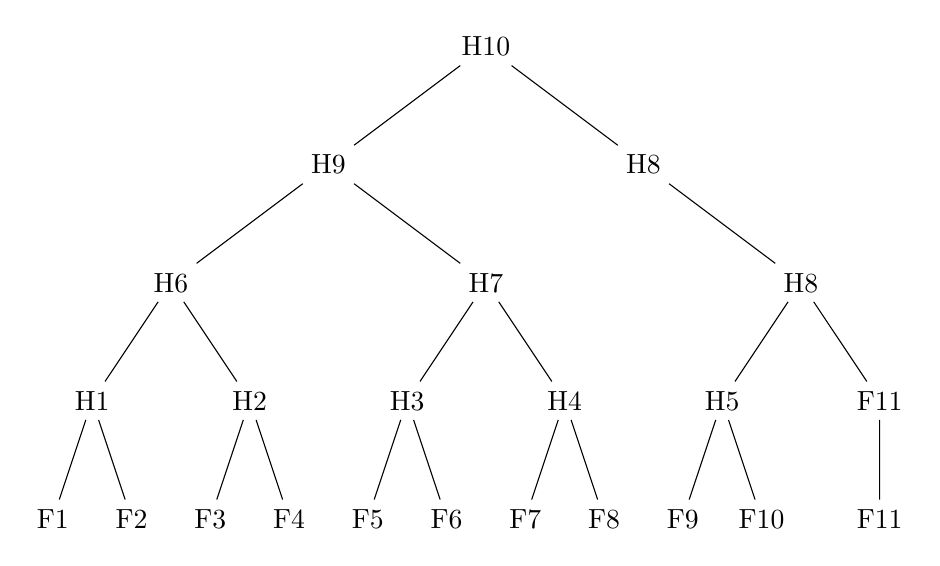
\begin{tikzpicture}[level distance=1.5cm,
        level 1/.style={sibling distance=4cm},
        level 2/.style={sibling distance=4cm},
        level 3/.style={sibling distance=2cm},
        level 4/.style={sibling distance=1cm},
        ]
        \node { H10 }
            child { node { H9 }
                child { node { H6 }
                    child { node { H1 } 
                        child { node { F1 } }
                        child { node { F2 } }
                    }
                    child { node { H2 } 
                        child { node { F3 } }
                        child { node { F4 } }
                    }
                }
                child { node { H7 }
                    child { node { H3 } 
                        child { node { F5 } }
                        child { node { F6 } }
                    }
                    child { node { H4 } 
                        child { node { F7 } }
                        child { node { F8 } }
                    }
                }
            }
            child { node { H8 }
                child [missing]
                child { node { H8 }
                    child { node { H5 } 
                        child { node { F9 } }
                        child { node { F10 } }
                    }
                    child { node { F11 } 
                        child { node { F11 } }
                    }
                }
            };
    \end{tikzpicture}
    \caption{Simple Merkle Tree Example}
    \label{fig:merkle_example}
\end{figure}

\subsubsection{Validation}

The validation can be either performed only on the initialization fragment or on at least one fragment in conjunction with the initialization fragment.

The initialization segment contains the C2PA manifest packaged in a \texttt{uuid} BMFF box. In a fragmented BMFF context this manifest must contains the aforementioned \texttt{c2pa.hash.bmff} Assertion. To verify the initialization segment one has to read the C2PA manifest and use the included hash exclusion ranges to recreate the hash of the initialization segment. If this hash is equal to the one found in the manifest then the initialization segment is validated as trustworthy.

Each fragment also contains a \texttt{uuid} box. However, the fragments only contain a CBOR-encoded data structure which holds information required for validation: the proof \texttt{hashes}, the \texttt{local\_id} and \texttt{unique\_id} and the \texttt{location} on that particular Merkle Tree, shown by the Rust structure BmffMerkleMap in \Cref{code:bmff_merkle}. The two IDs are required to identify the corresponding Merkle Tree from the C2PA manifest in the initialization segment and the location is the leaf index of the fragment which is needed to determine whether this fragment is the left or right child of their parent node.

\begin{minipage}{\linewidth}
\begin{lstlisting}[caption={BmffMerkleMap Rust Definition}, label=code:bmff_merkle, language=Rust, captionpos=b]
    pub struct BmffMerkleMap {
        // unique ID
        pub unique_id: u32,
        // local ID
        pub local_id: u32,
        // leave index on the Merkle Tree
        pub location: u32,
        // proof hashes
        pub hashes: Option<VecByteBuf>,
    }
\end{lstlisting}
\end{minipage}

The validation of a fragment requires the successful validation of the accompanying initialization segment. First step of the validation is calculation of the data hash using the exclusion ranges according to the C2PA manifest. Next the proofs are used in sequence to reconstruct the Merkle Tree. This is done by first determining whether the fragment is a left or right node. The \texttt{location} values begin at zero indicating that an even \texttt{location} representing a left node and an odd \texttt{location} a right node. The first proof is the direct sibling of the fragment. Then the first parent can be calculated using the first proof and the information of \texttt{location} by concatenating the two hashes (left + right) and hashing the result again using the algorithm specified in the C2PA manifest. This is repeated with the newly created hash and the next proof until all proofs have been used. The final hash resulting from these steps should equal one of the hashes located in the corresponding Merkle Tree from the C2PA manifest. If that is the case the fragment has been validated as trustworthy \footnote{BMFF-Based Hash Validation: \url{https://c2pa.org/specifications/specifications/2.0/specs/C2PA_Specification.html\#_validation}}. A simplified version of the can be seen in pseudo code in \Cref{alg:validate}.

\begin{algorithm}[H]
    \begin{algorithmic}[1]
        \Require $refTreeLayer$ \Comment{read from C2PA Manifest}
        \Require $location$ \Comment{read from Fragment}
        \State $fragHash \gets hash(fragment)$
        \ForAll{$proof \gets fragment.proofs$}
            \If{location is right}
                \State $fragHash \gets hash(proof + fragHash)$
            \Else
                \State $fragHash \gets hash(fragHash + proof)$
            \EndIf
        \EndFor
        \If{fragHash in refTreeLayer}
            \State fragment is valid
        \Else
            \State fragment is invalid
        \EndIf
    \end{algorithmic}
    \caption{Validating a Fragment}
    \label{alg:validate}
\end{algorithm}

\subsection{Signing Fragmented BMFF Files\label{sec:sign_bmff}}

\todo[inline]{explain the existing signing}

\section{Concurrent Approaches}

\todo[inline]{DRM?}
\todo[inline]{Fingerprinting?}
\todo[inline]{Watermarking?}
\todo[inline]{other live pocs}